\chapter{Introduction}

Explain the reason why there are two and how they compare to each other.



%% TODO: Short intro here
\subsection{Threat Model}
% Taken and tweaked from disksec
From the perspective of verification, we would like to have confidence
that the file system is secure purely based on the file system's security
specification.  This means that we have to treat the developer of the
file system with an adversarial mindset.  This subsumes all possible
bugs that a well-meaning but error-prone developer might introduce into
the implementation as well as any implementation that is designed to be exploited.

As a result, our threat model is that the adversary both develops the
file system and runs an adversarial application on top of the file system
in an attempt to obtain confidential file data.  However, the adversary
does provide a proof that their file-system implementation meets our
security specification.  The potential victim runs on top of the same
file system but sets their permissions so that the confidential files
are not accessible to the adversary's process.  Our goal is to ensure
that the security specification is so strong that it prevents leaks even
when the file-system developer is colluding with adversarial processes
running on top of the file system.

Our threat model is focused on proving that the file-system implementation has
no confidentiality bugs, rather than proving the absence of bugs in the
environment outside of the file system. Thus, we assume that our model
of how the file-system implementation executes is correct.  That is, we are not
concerned with bugs in unverified software or hardware outside of the file
system, or users mounting malicious disk images.  We do prove that
\texttt{mkfs} produces a correct image, but ensuring confidentiality on top of an
intentionally corrupted file system image is difficult, even without formal
verification. 

%%% Disksec doesn't reason about time. ConFrm reasons about it at coarse granularity.
%%% TODO: I will add these to their respective chapters

%We also do not reason about timing channels, as we do not model time.

%We only reasoning about time in a coarse granularity, 
%i.e. number of operations executed. Each operation having having different execution time 
%(e.g. a memory write is much faster than a disk write) is out of scope of this work.


% Taken from disksec
\subsection{Challenges}
\label{s:goal:chal}

The most difficult aspect of formally proving the security of a file system lies
in guaranteeing confidentiality.  This is difficult for several reasons.

\paragraph{Two-safety.}
First, proving confidentiality is more difficult than
proving functional correctness: as mentioned earlier, confidentiality
is a two-safety property.  Functional correctness is a one-safety
property because a violation of functional correctness can be demonstrated
by a single execution.  For instance, if an application wrote one byte to
a file and then read back a different byte, this single execution shows
that the file system is incorrect.  Thus, functional correctness
of a file system is a theorem that says that all executions meet the
spec (i.e., there are no such violations).  Integrity properties,
such as ensuring that one user cannot corrupt another user's data,
are an example of a one-safety functional-correctness property and can
be handled using standard verification techniques.

In contrast, demonstrating a violation of confidentiality requires
two executions, where the results observed by an adversary differ depending on
the secret data.
%% %% TODO: We don't do this though. Maybe find a better example for this?
For instance, consider a file system with block-level deduplication that
also exposes the number of free blocks.  An adversary who wants to
learn the contents of a victim's file could write their guess for the
victim's block into the adversary's own file and then check whether
the number of free blocks stayed the same or decreased.  If the file
system implemented deduplication across users, this attack allows an
adversary to learn whether their guess block was already present in the
file system, thus inferring whether the victim has that data.

In the above example, looking at a single execution does not allow one
to directly conclude that data was leaked, because the system appears
to be functioning correctly.  Determining that data is leaking requires
one to consider a pair of executions, in which the adversary performs
the same operations, but the confidential user data is different.
If these two executions produce different adversary-observable results,
the adversary is able to infer information about confidential data.

By stating confidentiality as a two-safety property, the above
deduplication example would violate confidentiality, and thus could not
appear in an implementation that was proven to achieve confidentiality.
Specifically, suppose the starting states of the two executions differed
in the contents of a confidential file, where in one execution the file
matched the adversary's guess and in the other execution it didn't match.
In this case, the number of free blocks returned by the adversary
would differ in the two executions, which would not be allowed by the
confidentiality definition.

\paragraph{Nondeterministic specifications.}
Another complication in proving confidentiality lies in the fact
that many specifications, including those in the file system, are
nondeterministic.  Some nondeterminism is unavoidable because file
systems must deal with crashes (e.g., due to power failure), which can
occur at any time.  Thus, it is impossible to
know what are the exact contents of the disk after a crash; the on-disk
state could reflect any prefix of the writes issued by the file system.
Modern disks complicate this situation even further by buffering writes
in memory inside the disk controller; as a result, the writes can be
made durable out-of-order, and the state of the disk after a crash might
reflect some out-of-order writes.  Even in the absence of crashes, the
file system implementation may want to use randomness (e.g., to randomize
directory hash tables), which makes the execution non-deterministic.

Other nondeterminism comes from specifications that hide irrelevant
details.  For instance, the inode allocator in the file system does
not specify which precise inode number will be returned; instead,
its specification simply states that it will return
\emph{some} inode number that is not already in use.

Any nondeterminism is a potential leak of confidential data.  The
nondeterministic specification of the block allocator from above does not
preclude the allocator from leaking confidential data, because it could,
in theory, choose the next inode number based on the confidential contents
of files, without violating its specification (i.e., still returning some
unused inode number).

Even the nondeterminism associated with the state of the disk
after a crash can be taken advantage of by an adversarial file-system
implementation to leak data.  For instance, a high-performance
file-system specification allows the file system to delay flushing data
to disk.  An adversarial implementation could choose whether to flush
data immediately or defer the flush based on one bit of confidential
data from a victim's file.  To take advantage of this, an adversary
could wait for the system to crash and, after the crash, check whether
any writes appear to have been lost.  If so, the adversary concludes
the file system must have deferred the writes, which would have only
happened if the confidential bit was zero.  This, in turn, can allow
the adversary to infer confidential bits.

\paragraph{Non-uniform outcome probabilities.}
Another possibility of leaking confidential data
arises because standard nondeterministic noninterference
captures what \emph{might} be possible, but an adversary may have
more precise information about the actual \emph{probabilities} of
different outcomes. A simple example of this weakness can be seen below: 

\begin{figure}[ht]
    \centering
\begin{verbatim}
if (random_bit() = 1)
  return secret_bit
else
  return random_bit()
\end{verbatim}
    \caption{Example of a noninterfering program that leaks information via return value frequencies}
    \label{fig:Frequency_Leaking_Program}
\end{figure}

This code leaks the secret bit 50\% of the time and outputs a random bit 50\% of the time. It is also important to note that it can output 0 or 1 independently of the secret value. This way, any (state, return) pair represents a successful execution. 

Let’s say that two states are equivalent if they are the same for their non secret parts. This makes all states equivalent to each other in our example. Since any pair of state and return value is a valid execution, it is possible to find another execution from a related state with same return value. Therefore, This implementation satisfies the nondeterministic noninterference definition. 

\begin{figure}[ht]
    \centering
    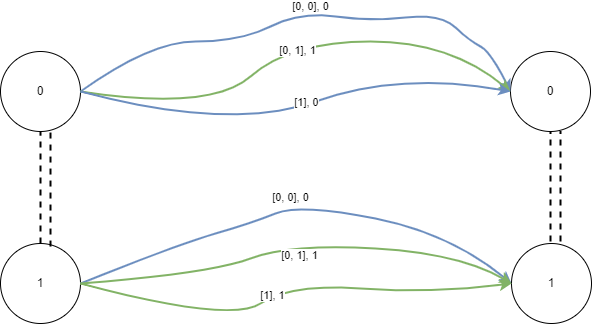
\includegraphics[scale=0.5]{templates/figures/matching-paths.png}
    \caption{Every execution matches with the execution of the same color.\\
    Numbers in brackets denote generated random bits. \\The number following the brackets denotes the return value.}
    \label{fig:NI_Matching_Paths}
\end{figure}

Although the above program satisfies the definition, the secret bit can be determined via the observed frequency of repeated calls. When we look at the frequencies of output values, we can see that they correlate with the value of the secret bit. \\

\begin{tabular}{| c | c | c |}
	\hline
	Secret bit & Output 0 \% & Output 1 \% \\
	\hline
	0 &	75\% & 25\% \\
	\hline
	1 &	25\% & 75\% \\
	\hline
\end{tabular}\\

Any adversary who can observe the output of the function sufficiently many times can infer the value of the secret bit with high confidence. These types of vulnerabilities are not limited to usage of randomization. They also manifest themselves when there are random events such as crashes that can affect the behavior of the system.


\paragraph{Indirect disclosure.}
Yet another complication with confidentiality is that an adversarial
file system might not immediately leak confidential data.  For example,
an adversarial file system may wait for a legitimate user to read
confidential data, at which point the file system would be allowed to
access this data, since it has to return it to the user.  However, in
addition to returning this data, an adversarial file system could also
stash away a copy of it, so that the adversary can later retrieve it.
For instance, the file system could change the order of entries in an
on-disk directory structure, or change the allocated inode numbers or
block numbers, based on the confidential data that it wants to leak.
Preventing this attack is difficult because the adversarial file system
appears to have legitimate access to the user's data when operating on
behalf of that user.

\paragraph{File-system complexity.}
Finally, file systems are complex software.  Linux ext4, for
instance, consists of approximately 50,000 lines of code.  Even the simple
verified DFSCQ file system consists of thousands of lines of executable
code~\cite{chen:dfscq}.  The proofs of functional correctness for DFSCQ
are already tens of thousands of lines of Coq code.  The complexity of
proving two-safety, which is a more challenging property, could easily
spiral out of control.
